

\section{Simulation Results}\label{se:simResults}

Figures \ref{figLPMvsTrunc} and \ref{fig:pdfAndRMSeVStruncTime} compare the LPM with and without truncation of the impulse response. They were obtained from simulations on 
the system described by the following simulation equations, which are relevant to the LPM outlined in Section \ref{se:LPMFRFest}:
\begin{subequations}
\label{eq:systemSimulations}
\begin{align}
y_0(t)  &= 1.5371y_0(t-1)    -0.9025y_0(t-2) + u(t)
\\
y(t) &= y_0(t) + e(t),
\end{align}
\end{subequations}
where $e(t)$ is a white noise sequence, such that the SNR of the output signal is 18.3~dB.

\begin{figure}[tbh] %top bottom here
\centering

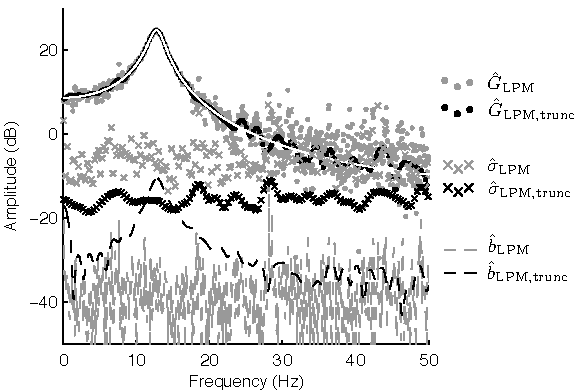
\includegraphics[scale=0.9]{figLPMvsTruncWlegend}

\caption{Comparison of the LPM and Truncated LPM estimates of the FRF for an SNR of 18.3~dB. The gray plots pertain to the LPM estimate without truncation, the black ones to the LPM with truncation (trunc). Dots: FRF estimates $\hat{G}$. Crosses: sample standard deviations $\hat{\sigma}$. Dashed lines: bias $\hat{b}$. White line: the true system $G_0$.}
\label{figLPMvsTrunc}
\end{figure}

In Figure \ref{figLPMvsTrunc} one observes the following:
\begin{itemize}
\item
a decrease of the variance on the truncated estimate of about 10~dB,  i.e. a decrease of the black crosses, compared to the gray ones, is observed. %i.e. a decrease of the black crosses w.r.t.~the gray ones is observed.

\item 
the error on the truncated LPM estimate is strongly correlated over the frequency. This must be taken into account when formulating a maximum likelihood parametric estimator of the system.	

\item
an increase of the bias of the truncated estimate, especially in the vicinity of the resonance frequency. Still, this bias lies below the variance of the non-truncated estimate. As such, for a single experiment, the increase in bias still yields a better estimate when truncation is invoked. % \JL{when performing the truncation}.

This bias depends on the time instant at which the truncation is performed, as discussed below.

\end{itemize}

\begin{figure}[htb] %  figure placement: here, top, bottom, or page
   \centering
    %\setlength\figureheight{0.45\columnwidth}
    %\setlength\figurewidth{0.7\columnwidth}
	%% This file was created by matlab2tikz.
%
\begin{tikzpicture}

\begin{axis}[%
width=0.951\figurewidth,
height=\figureheight,
at={(0\figurewidth,0\figureheight)},
scale only axis,
xmode=log,
xmin=10,
xmax=2048,
xtick={10,100,1000},
xticklabels={\empty},
xminorticks=true,
ymin=0,
ymax=500,
ytick={  0, 100, 200, 300, 400, 500},
ylabel={Number of realizations},
axis x line*=bottom,
axis y line*=right
]
\addplot[histogramSmootherFTest] plot table[] {\thisDir/figs/pdfs-3.tsv};
% \addplot[forget plot,color=white!15!black,solid,line width=2.0pt] table[] {\thisDir/figs/pdfs-4.tsv};

\addplot[histogramSmootherExpFit] plot table[] {\thisDir/figs/pdfs-5.tsv};
% \addplot[forget plot,color=white!15!black,solid,line width=2.0pt] table[] {\thisDir/figs/pdfs-6.tsv};

\end{axis}


\begin{axis}[%
width=0.951\figurewidth,
height=\figureheight,
at={(0\figurewidth,0\figureheight)},
scale only axis,
xmode=log,
xmin=10,
xmax=2048,
xminorticks=true,
xlabel={Truncation Time $\truncTime$ \axisunit{samples}},
ymin=0,
ymax=2.5,
ytick={  0, 0.5,   1, 1.5,   2, 2.5},
ylabel={RMS Error \noaxisunit},
legend style={legend cell align=left,align=left,draw=black}
]
\addplot [mainCurve] table[]{\thisDir/figs/pdfs-1.tsv};
\addlegendentry{RMS Error};

\addplot [pointOfInterest] table[]{\thisDir/figs/pdfs-2.tsv};
\addlegendentry{Theoretical optimum};

% \addlegendimage{empty legend}
% \addlegendentry{\textbf{Histograms using:}};

\addlegendimage{histogramSmootherFTest}
\addlegendentry{$F$-test};

\addlegendimage{histogramSmootherExpFit}
\addlegendentry{Exponential fitting};



\end{axis}
\end{tikzpicture}%

	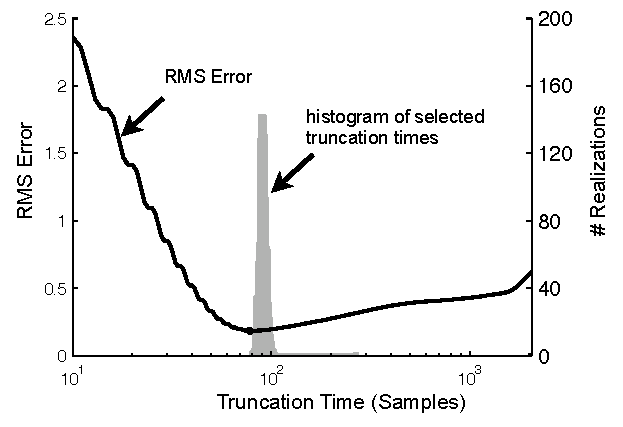
\includegraphics{HistogramExpFitting.pdf}
 \caption{Black full line (left hand side y-axis (ordinate)): total RMS error as a function of the truncation time (the single black dot is the minimum of the RMS). Gray histogram (right hand side y-axis (ordinate)): selected truncation times for 1000 noise realizations by the exponential fitting methods.}

   \label{fig:pdfAndRMSeVStruncTime}
\end{figure}

In Fig. \ref{fig:pdfAndRMSeVStruncTime}, the black graph is the RMS error of the estimated FRF (without the DC value) as a function of the time $t_\mathrm{trunc}$ at which the impulse response is truncated. Its minimum is indicated by a black dot, to the left of which a steep increase is observed. This is due to a bias error. To the right hand side of the minimum, the RMS error increases very gradually, due to an increase of the noise variance.

A good practice would be to truncate the impulse response at the minimizer (black dot) of the RMS error. However, it should be noted that this minimizer is unknown in practice, because it would require
the true FRF.

The truncation time is determined from the data as described in Section \ref{se:truncImpulseResp}. This was done on $1000$ realizations of the noise, and depicted in Figure \ref{fig:pdfAndRMSeVStruncTime} by the histogram.
Clearly, the method for selecting the truncation time $t_{\mathrm{trunc}}$ has a good overall performance, based on the mode of its distribution. A closely grouped set of values for $t_{\mathrm{trunc}}$ is obtained around the $90^{\text{th}}$ sample, without significant outliers.

From the plot, we can conclude that the RMS error increases rapidly when $t_{\mathrm{trunc}}$ is smaller than the optimal.
On the other hand, selection of a value of $t_{\mathrm{trunc}}$ that is too large, is not nearly as detrimental to the modeling error.
The graph also shows that the RMS error of the model can be decreased from $0.62$ (without truncation) to $0.18$ when the optimal truncation is applied. Also, one observes a low sensitivity of the RMS error w.r.t.~$t_\mathrm{trunc}$, when truncating at times beyond that optimum. Therefore, a somewhat conservative truncation method is still likely to yield a close to optimal result.

